\documentclass[a4paper,11pt]{report}
\usepackage[english]{babel}
\usepackage{graphicx} 
\usepackage{pdfpages}
\usepackage{fancyvrb}
\bibliographystyle{unsrt}
\usepackage{url}
\usepackage{listings}
\usepackage{natbib}
\usepackage[cyr]{aeguill}
\usepackage{pdflscape}
\usepackage{fullpage}
\usepackage{algorithm}
\usepackage{algorithmic}
\usepackage{textcomp}

\usepackage{enumitem}


% Turtle box
\definecolor{olivegreen}{rgb}{0.2,0.8,0.5}
\definecolor{grey}{rgb}{0.5,0.5,0.5}
\lstdefinelanguage{ttl}{
sensitive=true,
morecomment=[l][\color{grey}]{@},
morecomment=[l][\color{olivegreen}]{\#},
morestring=[b][\color{blue}]\",
keywordstyle=\color{cyan},
morekeywords={version,owl,rdf,rdfs,xml,xsd,dbpedia,dbo,str,sso,scms,fr,ld}
}
\lstset{
        basicstyle=\ttfamily\scriptsize,
        upquote=true,
        showspaces=false,
        showstringspaces=false,
        showtabs=false,
        tabsize=2,
        frame=none,
        breaklines,
        numbers=none,
        framexleftmargin=2mm,
        xleftmargin=2mm,
}

\hyphenation{u-bi-qui-ty}
\hyphenation{a-llows}
\hyphenation{on-to-lo-gy}



%%%%%%%%%%%%%%
%DOCUMENT BEGINS HERE 
%%%%%%%%%%%%%%%%


\begin{document}

\begin{titlepage}
\begin{center}

\includegraphics[width=5cm]{EURECOM_logo_quadri}
\\[3cm]
\textbf{\Huge{Activity Report}}
\\[2cm]
\textbf{\textsc{\LARGE{Year: 2013-2014}}}
\\[0.5cm]
\LARGE{Jose Luis Redondo Garcia}
\\[0.5cm]
\small{EURECOM-Multimedia Communications}
\\
\large{Institut Mines-Telecom}
\\
\large{September 11th, 2014}
\\[8cm]
\columnsep3cm
\begin{tabular}{p{8cm} p{8.5cm}}
\small{\textbf{Supervisor:}\newline
Rapha\"el Troncy} 
&
\small{\textbf{EURECOM\newline Multimedia Department}}
\end{tabular}
\end{center}
\end{titlepage}

% \tableofcontents

\chapter*{Introduction}
%\addcontentsline{toc}{chapter}{Abstract}

This report presents the research work carried out by \textbf{Jos\'e Luis Redondo Garc\'ia} as a PhD student of the doctoral school Telecom ParisTech during the period from September 2013 to August 2014. These activities havw been done at EURECOM, under the supervision of Rapha\"el Troncy and in the context of the EU LinkedTV project.

The sections in this document are organized as follow: first, the research problem in our thesis: \textbf{"Interacting with hypervideos semantically enriched''} is explained. We also list the different contributions achieved so far. Then, we present the publications and the information about the research project we are currently working. Finally, we outline the future work.

%\section*{Contents}

\chapter*{Research Problems}

The amount of multimedia content available is huge: there are billions of pictures and videos spread in very different ecosystems that keep growing. Since each of those ecosystems has is own peculiarities, it is not easy to identify which media items are relevant in a particular context, and how they can be effectively consumed or re-used by users. Television content constitutes a subset of this multimedia world where the presence of isolated ecosystems becomes even more obvious: broadcasters such as the German RBB or the French TF1 are the owners of tons of television content that are not conveniently exposed and interlinked with the rest of the world.

Multimedia content is rapidly increasing in scale and ubiquity but it still remains largely poorly indexed and unconnected with other related media from other sources. The current state of the TV domain clearly reflects this fact: there are no clear approaches for going further than a simple PC-like browsing experience on a full screen. Users wish to have new functionalities such as getting access to information not explicitly present in the television content itself, like browsing from a local news show to an open government data portal about a particular location in order to understand voting patterns, or learning more about animals and plants shown in a nature documentary without leaving that show.

The information available in social platforms is growing and becoming more and more attached to television programs. Filtering this massive amount of data and trying to make sense out of it is an extremely challenging task due to the heterogeneity and dynamics of the information. Such an analysis is, however, very valuable for explaining or illustrating what is going on in a video using similar audiovisual content or encyclopedia knowledge, for completing missing information, or for providing other users point of view about the same fact or topic.

Other open issue is the way those media items are described. In most of the cases, the content is considered like an unitary piece that does not need to be further fragmented. However, in many situations, a more fine-grained decomposition of the media resource is needed, in order to point to particular fragments where something of interest is happening. The broad variety of non-interoperable standards for representing those descriptions, such as TV-Anytime\footnote{\url{http://tech.ebu.ch/tvanytime}} or MPEG-7\footnote{\url{http://mpeg.chiariglione.org/standards/mpeg-7}}, has been largely recognized but they are not designed with Web principles in mind. There is a need of complementing seed video programs with additional resources on the Web, such as domain related web sites, encyclopedic sources or even conversation happening on social platforms. Below we summarize the various challenges that this new multimedia vision implies:
\begin{itemize}
\item How to semantically annotate multimedia content in the Web.
\item How to segment multimedia content in meaningful fragments that could be interlinked with relevant information in the LOD cloud.
\item How to enrich multimedia content and make sense of a collection of media items.
\end{itemize}


\chapter*{Contributions}
\section*{Named Entity Expansion} \label{expansion}

Relying on subtitles to extract named entities that can be used to index fragments of a program is the most extended method for semantically annotate documents. However, this approach is limited to what is being said in a program and written in a subtitle, therefore lacking a broader context. In order to overcome this problem we take advantage of the power of non-structured documents combined with structured data coming from DBpedia to generate a much richer, context aware metadata of a particular type of television programs: the newscast. We demonstrate that we can harvest a rich context by expanding an initial set of named entities detected in a media fragment.

In addition sometimes entities spotted over a particular document are not disambiguated because the textual clues surrounding the entity are not precise enough for the name entity extractor, while in other cases, they are simply not mentioned in the transcripts while being relevant for understanding the story. This is an inherent problem in information retrieval tasks: a single description about the same resource does not necessarily summarize the whole picture of it. The named entity expansion operation relies on the idea of retrieving and analyzing additional documents from the Web where the same event is also described. By increasing the size of set of documents to analyze, we increase the completeness of the context and the representativeness of the list of entities, reinforcing relevant entities and finding new ones that are potentially interesting inside the context of that news item. The entire process is illustrated in Figure~\ref{fig:namedEntityExpansion}.

\begin{figure}[h!]
\centering
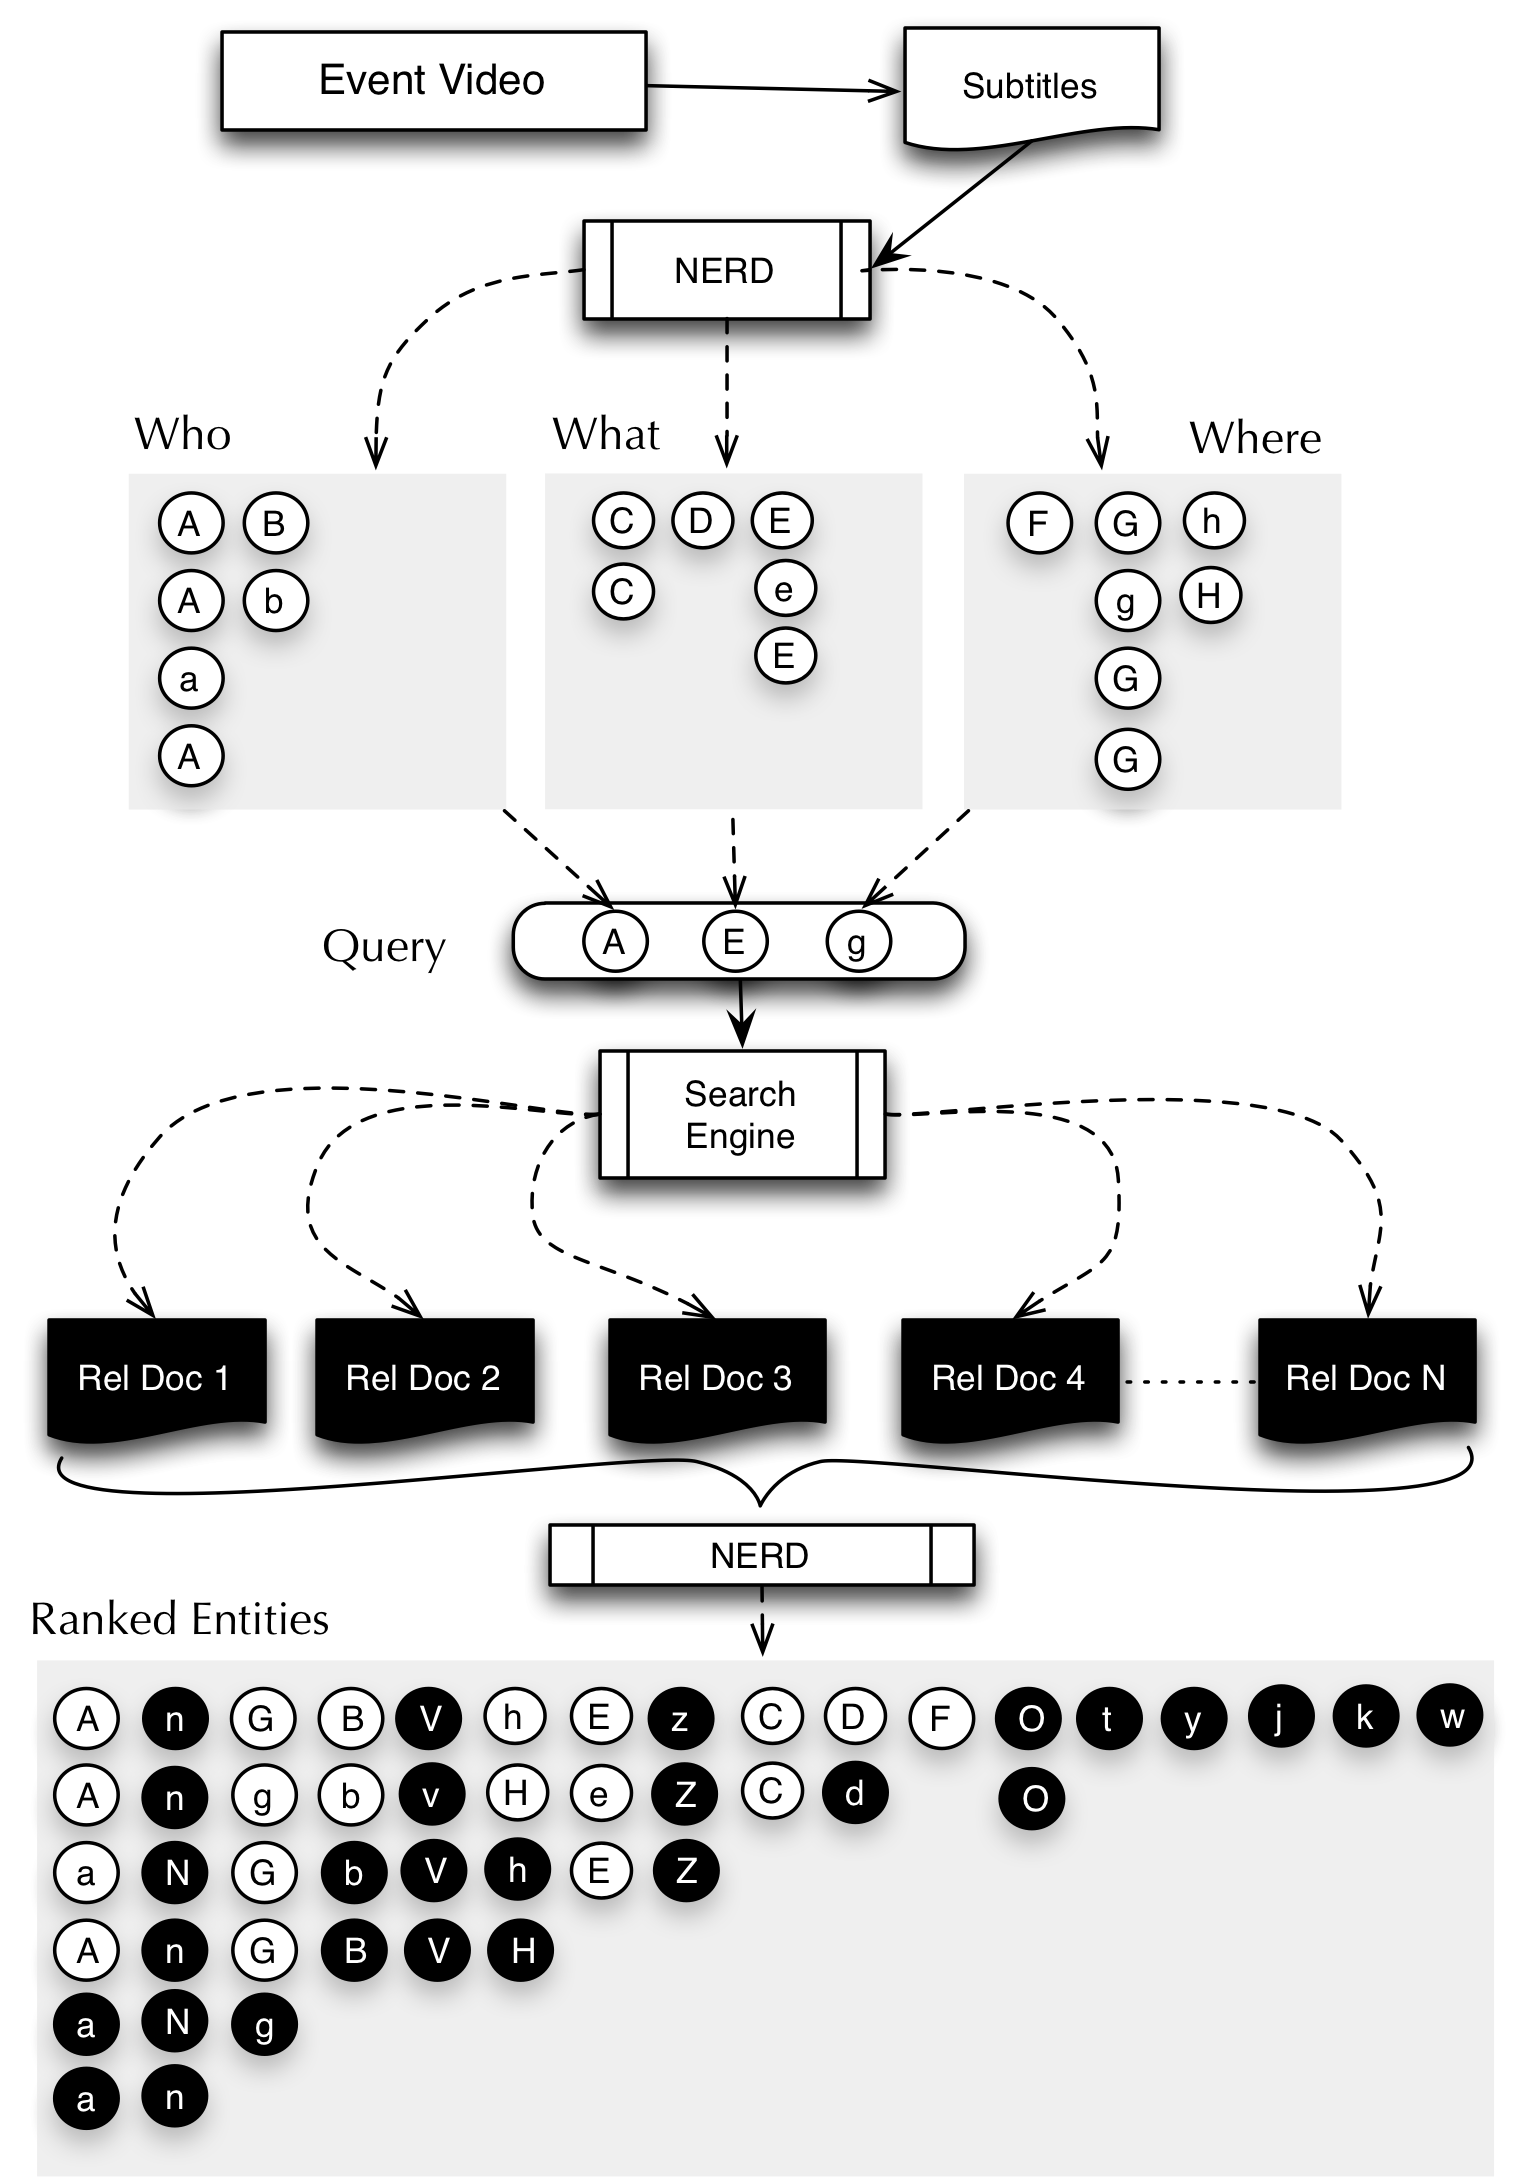
\includegraphics[width=0.5\textwidth]{figure/ExpansionDiagram}
\caption{Schema of Named Entity Expansion Algorithm.}
\label{fig:namedEntityExpansion}%\end{figure}
\end{figure}

First, we build a query based on the \emph{Five W's}, a popular concept of information gathering in journalistic reporting that captures the main aspects of a story: who, when, what, where, and why. The original entities are mapped to the NERD Core ontology, which considers 10 main classes: Thing, Amount, Animal, Event, Function, Organization, Location, Person, Product and Time. From those ten different categories, we generalize to three classes: the Who from \url{nerd:Person} and \url{nerd:Organization}, the Where from \url{nerd:Location}, and the What from the rest of NERD types after discarding \url{nerd:Time} and \url{nerd:Amount}. The When or so-called temporal dimension does not need to be computed since it is considered to be provided by the video publisher via legacy metadata. This query is injected into a document search engine where additional descriptions about the news event can be found.  The resultant documents (colored in black in the Figure~\ref{fig:namedEntityExpansion} will be further processed to increase the size of the collection and get additional insights about the news item.

In the next phase, the additional documents which have just been retrieved are now processed and analyzed in order to extend and re-rank the original set of entities and consequently get a better insight about the event. 
In order to calculate the importance of a particular concept within the entire corpora, we group the different appearances of the same instance and check their cardinality. This is not a trivial task since the same entity can appear under different text labels, contain typos or have different disambiguation URL's pointing to the same resource. We performed a centroid-based clustering operation over the instances of the entities. 

The final step consists of ranking the different named entity clusters obtained so far. To create this ordered list, we assigned a score to every entity according to the following features: relative frequency in the transcripts of the event video; relative frequency over the additional document; and average relevance according to the named entity extractors. Entities with a higher $relScore_{i}$ in the final classification are considered more representative for describing the context than the original entities. Furthermore, entities that originally have not been disambiguated can now have their corresponding URL if any of the similar instances appearing in the additional documents provide a link to a Web resource. The same occurs with incomplete or misspelled labels. Even some entities not spotted in the original transcripts but important in the context of the event are now included in the list of relevant items since they have been extracted from the collected documents.


\section*{Multimodal Annotation: Semantic and Visual Analysis} \label{semanticVisual}

Thanks to semantic media annotation the available knowledge about a particular multimedia content gets aligned with Web resources and consequently grows exponentially. But visual analysis results should not be underestimated since they are the only ones able to fully capture the exact essence of a multimedia content: which faces and objects are appearing on the screen at a certain moment, at which exact moment a particular scene is starting, how colorful is the depicted landscape... they are all aspects that can be uniquely detected via visual processing. Therefore semantic annotations can be complement with visual analysis results in order to further specify what is being happened on in a video content. 

\subsection*{From Named Entities to Visual Concepts}

Linking visual concepts to semantic units was a key challenge of this work. Taking as input visual cues specified by humans, we have run keyword and named entity extraction operations by using Alchemy API\footnote{\url{http://www.alchemyapi.com/}}. After that, we have tried to align every spotted keyword with some LSCOM concepts (currently, a subset of more than one hundred items currently has been considered) by applying  semantic word distance based on Wordnet\footnote{\url{http://wordnet.princeton.edu/}} synsets.

\subsection*{Indexing Scenes and Visual Concepts}

Under the context of the LinkedTV project videos are analyzed following different visual techniques. We performed concept detection on the key-frames of the video, Optical Character Recognition (OCR) for text localization, and keyword extraction over the provided subtitles. We grouped the predefined video shots into bigger segments (scenes), based on the visual similarity and the temporal consistency among them. All those algorithms are publicly exposed via a REST interface~\footnote{\url{ http:///pronto.iais.fraunhofer.de:8000}}. 

We used the search framework Solr~\footnote{\url{http://lucene.apache.org/solr/}} in order to index all available data, at different granularities: video level, scene level, shot level, subtitle block level, speech segments from transcripts. Hence, searches can be performed at a chosen granularity. The results of the search task allow to notice than given the same conditions and regarding the pure textual information, subtitles perform significantly better than any of the transcripts, which is an expected outcome. It is also interesting to note that using the visual concepts in the query increases the results for all measures. This probes the efficiency of combining semantic and visual concepts in search operations.

In the same line, we extended the search operation in order to accept as input media fragments themselves in order to switch to an hyperlinking approach. In this situation the query is obtained by leveraging in the corresponding annotations for the input media fragment: subtitles, keywords and visual concepts scores are extracted from the keyframes contained in the anchor. By experimenting with different media fragment granularities, we discovered that our scene segmentation approach obtains the best performance when proposing related content. This probes the importance of a good segmentation algorithm, and opens a window to potential improvements for refining way segmentation results complements semantics annotations and vice-versa.


\section*{Named Entity Reranking using DBPedia}

The entities attached to one media fragments can be further refined and ranked by using the knowledge available in DBpedia. During this academic year we have studied how to rely in the powerfulness of structured sources to reinforce the important entities and finding relevant predicates between them.

\subsection*{Generating DBpedia paths}

Before we filter the relations between resources to reinforce important entities, the candidate resources to be included in relations are pre-ranked. They are pre-ranked according to ``popularity'' and ``rarity''which are essential components in the original PageRank algorithm and which is used to sort candidate related nodes in the EiCE~\footnote{\url{http://www.everythingisconected.be}}. The implementation of the EiCE takes the relations into account by making use of the Jaccard coefficient to measure the dissimilarity and assign random walks based weight able to highly rank more rare resources, and guaranteeing that paths between resources prefer specific relations and not general ones.

\begin{figure}[h!]
\centering
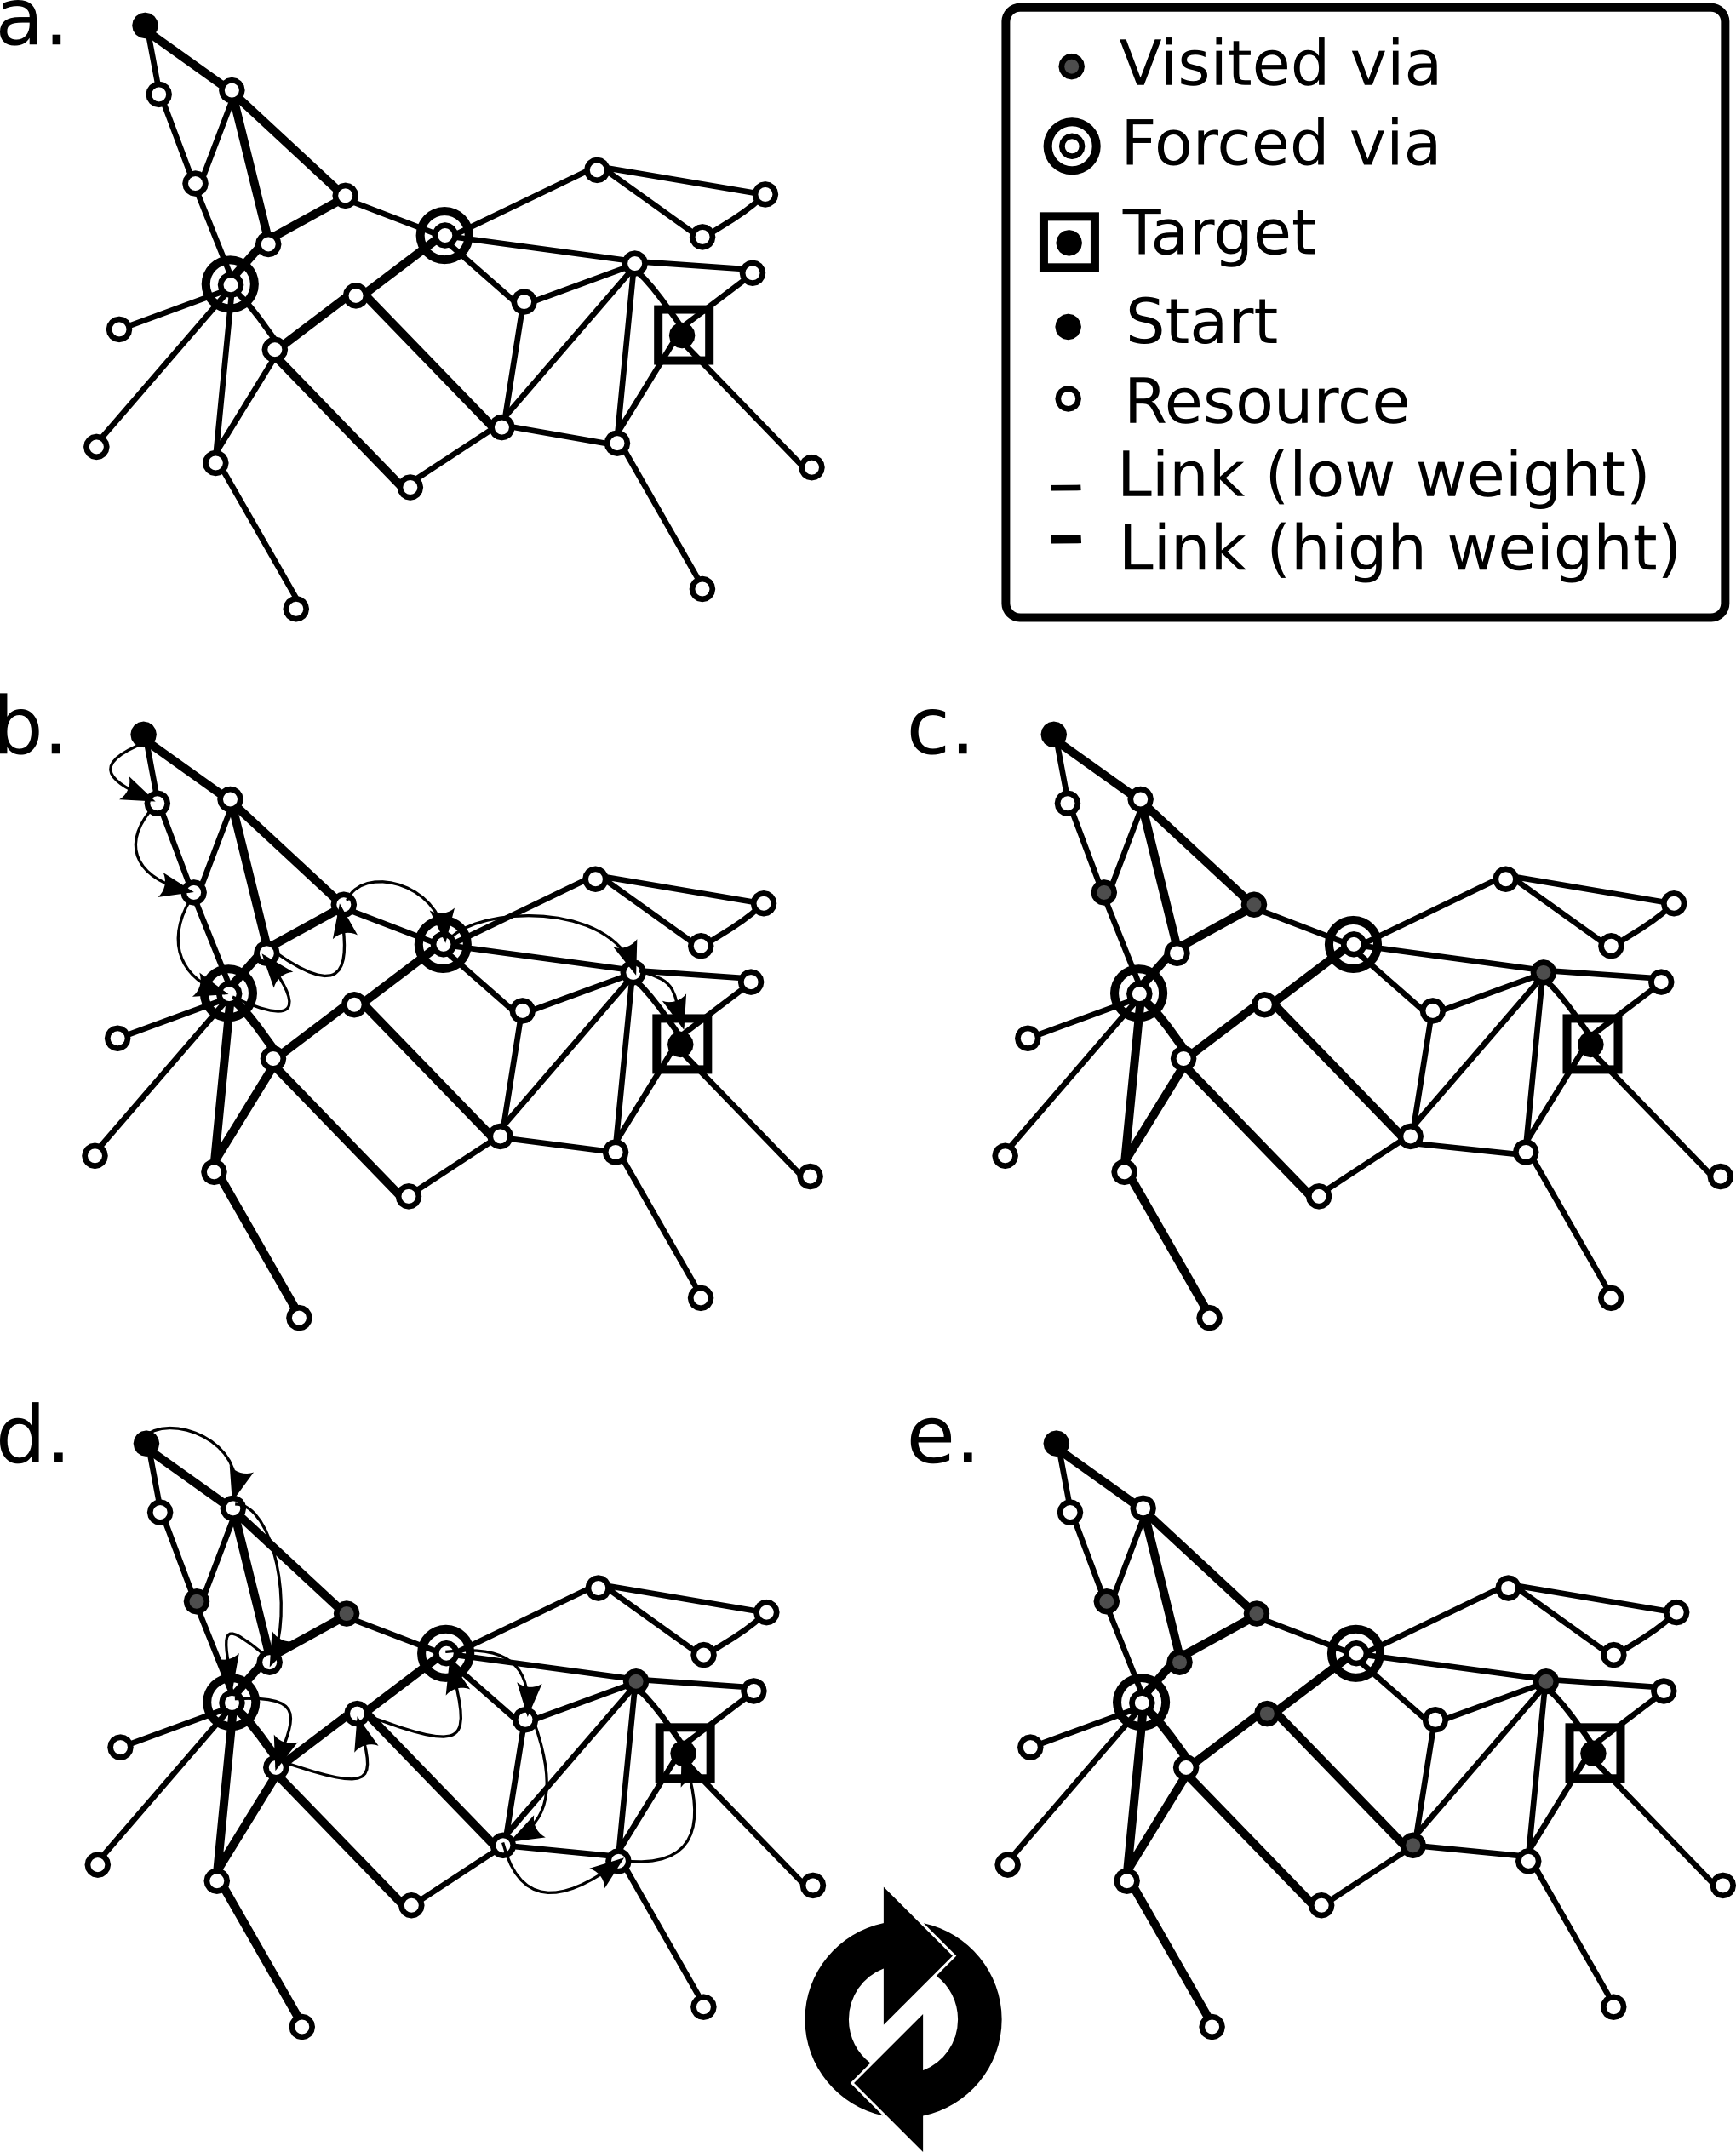
\includegraphics[width=0.5\textwidth]{figure/graphmultipatternmatching.png}
\caption{Pattern matching with multiple results using an iterative pathfinding process.}
\label{fig:patternmatching}
\end{figure}

\subsection*{Analyzing Relevant Paths}
In this step, the previous DPpedia path finding technique implemented is applied over the set of entities obtained via entity extraction and expansion. In particular, we calculate paths between all the possible pairs inside the set\textit{mainEntities}. Once all the possible paths have been retrieved, we perform various analysis for detecting which are the most frequent classes and predicates:
\begin{itemize}
  \item We detect the most frequent nodes.
  \item We find the most frequent properties. The edges (DBpedia properties) will determine which are the most relevant properties taking part in the context of this news item.
  \item We study the connectivity between nodes (Adjacency Matrix, where the distance between elements is the average length of the paths linking them)
\end{itemize}

The output is a re-ranked list of entities from the expansion entity set based on the paths found in DBpedia, the most important predicates and nodes inside the paths between pairs, and the adjacency matrix.

\section* {Newscasts Enrichment}
\label{newscasts}

People consume news from multiple sources, such as television, Web, radio and newspapers. For example, we watch the newscast on TV early in the morning to get an overview of the main news, we use the Web to keep track of the News throughout the day, and when we have some spare time we actively browse the Web to explore the news items that we are interested in. At the end of the day, our understanding about the news is a compendium of various information pieces coming from different sources, which complement each other and enrich our news experience. The problem is that in practice it is difficult and time consuming to manually gather all those insights together. Our research tackles this inconvenience by quickly offering extra information about the newscast organized in various dimensions which intend to illustrate all those details you watched but would like to further explore. 

Based on some user experience television studies conducted by collaborators at CWI~\footnote{\url{http://www.cwi.nl/}}, we have developed a service that intends to feeds newscast with relevant related document organized in different dimensions. This service acts as a hub where the viewers can access extra documents for complementing what is being told in the main news video. A similar logic to the one used for named entity expansion (the 5W's) is applied over the main entities coming from the expansion process for building custom queries in Google CSE, but operating over particular lists of Web resources. In contrast to traditional news aggregators that simply gather related documents, the results are organized around five different axes that intent to fulfill the viewer' needs. 

\textbf{Timeline.} Follows the news story throughout time by confectioning an list of ordered documents that includes the main antecedents of the present facts. For getting those document we rely on a query without any prior time constraint, which is created when including the most relevant entity from the Who, Was, Where inside the pattern ``The'' + entity + ``case''. 

\textbf{In other sources.} This section of the interface is dedicated to showing the selected news as it was reported in other newspapers, radio, or TV programs. We launch a query generated from the set of expanded entities by following exactly the same logic used during the entity expansion, over a curated list of resources including mainly Journals and television broadcasters Web sites. 

\textbf{Opinion.} This section is devoted to gathering opinions regarding the selected news item from different authors with a certain presupposed knowledge about the matter. The list of documents is obtained by executing the same query generated for dimension ``In other Sources'', but operating over a different list of curated resources that considers only subdomains specialized in opinion documents.

\textbf{Geo-localized information.} This section includes live feeds from Twitter API expressing people's remarks, comments and feelings filtered by subject and geo-location. We use the same textual query than in ``In other Sources'' dimension, but reducing the temporal dimension $t$ to the last 7 days from the current time, in order to see what the people is thinking about the particular news item.

\textbf{In depth.} Includes in depth coverage articles that offer a more extensive view about the seed news item. They documents under this dimension are obtained by combining the most relevant entity from the Who, Was, Where with the keyword ``in depth'' and removing any temporal restriction and extending the search domain to the entire Web. 

\subsection* {Companion Web Application for Navigating Newcasts}

LinkedTV News (see Figure~\ref{fig:DemoScreen}) is a second screen application for tablets that acts as a companion to viewers when watching the news broadcasts. Its main goal is to enrich television newscasts by integrating them with other documents and media via Web knowledge extraction techniques. It is designed to accommodate two viewing modes in terms of interaction: the so called passive and active modes. 

\begin{figure}[h!]
\centering
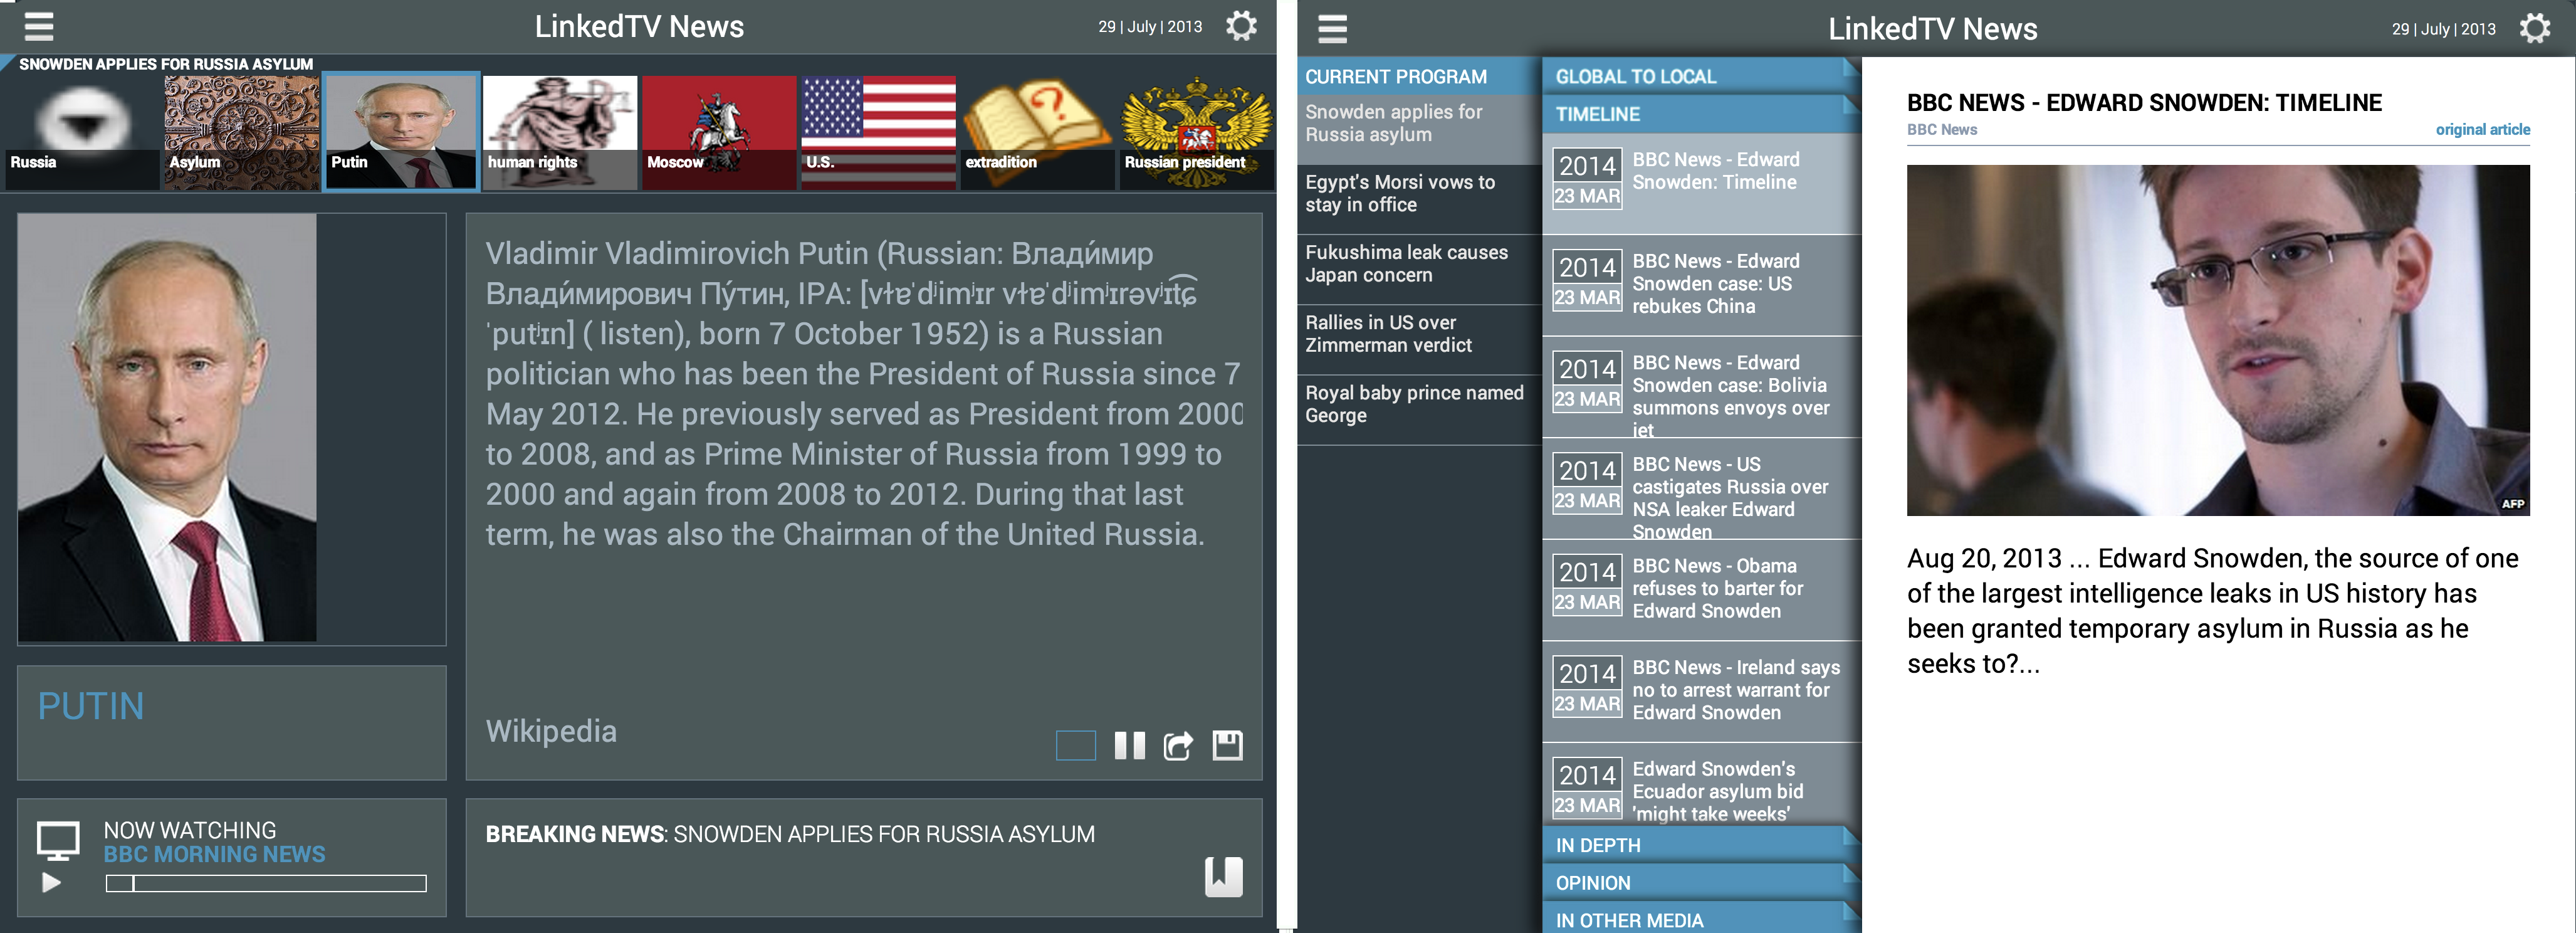
\includegraphics[width=1\textwidth]{figure/DemoScreen}
\caption{Demo screen captures corresponding to the (1) active mode and the (2) passive mode. Access the demo at \protect\url{http://linkedtv.project.cwi.nl/news/} for more details.}
\label{fig:DemoScreen}%\end{figure}
\end{figure}

In the passive mode the application operates as a second screen that is synced with the TV program. This mode supports the user with looking up factual information by presenting timed slides about the entities that occur in the news. As this mode requires no interaction it unobtrusively complements the lean back TV viewing experience. In the active mode the user actively explores that specific news item. In this mode the application contains articles from the Web that are related to the news item in different dimensions that were previously explained.

To reconstruct the semantic context associated with one particular news video, we have performed named entity expansion over the transcripts, since the set of entities obtained from a traditional named entity extraction operation is normally insufficient and incomplete for expressing the context of a news event. This step is crucial not only because it complements what the user is watching in every moment, but also because it generated the concepts that launch further enrichments in the active mode. 

\section* {Hotspots in Videos}
\label{hotspots}

We have developed an approach that leverages on visual analysis techniques and the knowledge present on the Web for identifying relevant fragments (called Hot Spots) inside educational online videos, in order to get a good overview about what is being told and promote the consumption of media clips at a higher level of granularity. 

Our approach performs a first segmentation by combining visual features and semantic units in transcripts (paragraph). The resultant video fragments are semantically annotated via Entity Extraction and Topic detection. By identifying consecutive chapters talking about similar topics and entities, we merge the initial segments into bigger and independent semantic media units. Finally we rank them, filter out the lower scored candidates, and propose a summary that illustrate the fragment and can be visualized on the dedicate media player. The algorithm has been applied in a set of educational TED talks. 

The obtained Hot Spots and their summaries are visualized in a user friendly MediaFragment URI \footnote{\fontsize{8pt}{1em}\selectfont \url{http://www.w3.org/TR/media-frags/}} compliant Web media player. The workflow to get Hot Spots available for a certain Ted talk goes like follows: after introducing a valid URL, we land in the video page from where the hot spot detection can be launch for the first time (see Figure~\ref{fig:demoScreenShots}a). When results are available, the corresponding fragments get highlighted on the timeline together with the label of the most relevant chapter annotation. This brief description can be extended to the broader set of main entities and topics in order to get a more exhaustive summary (see Figure~\ref{fig:demoScreenShots}c). Finally as shown in Figure~\ref{fig:demoScreenShots}d you can always relive that part of the talk you like the most or you would like to share with others. An online demo of the proposed solution is available at \url{http://linkedtv.eurecom.fr/mediafragmentplayer}.

\begin{figure}[h!]
\centering
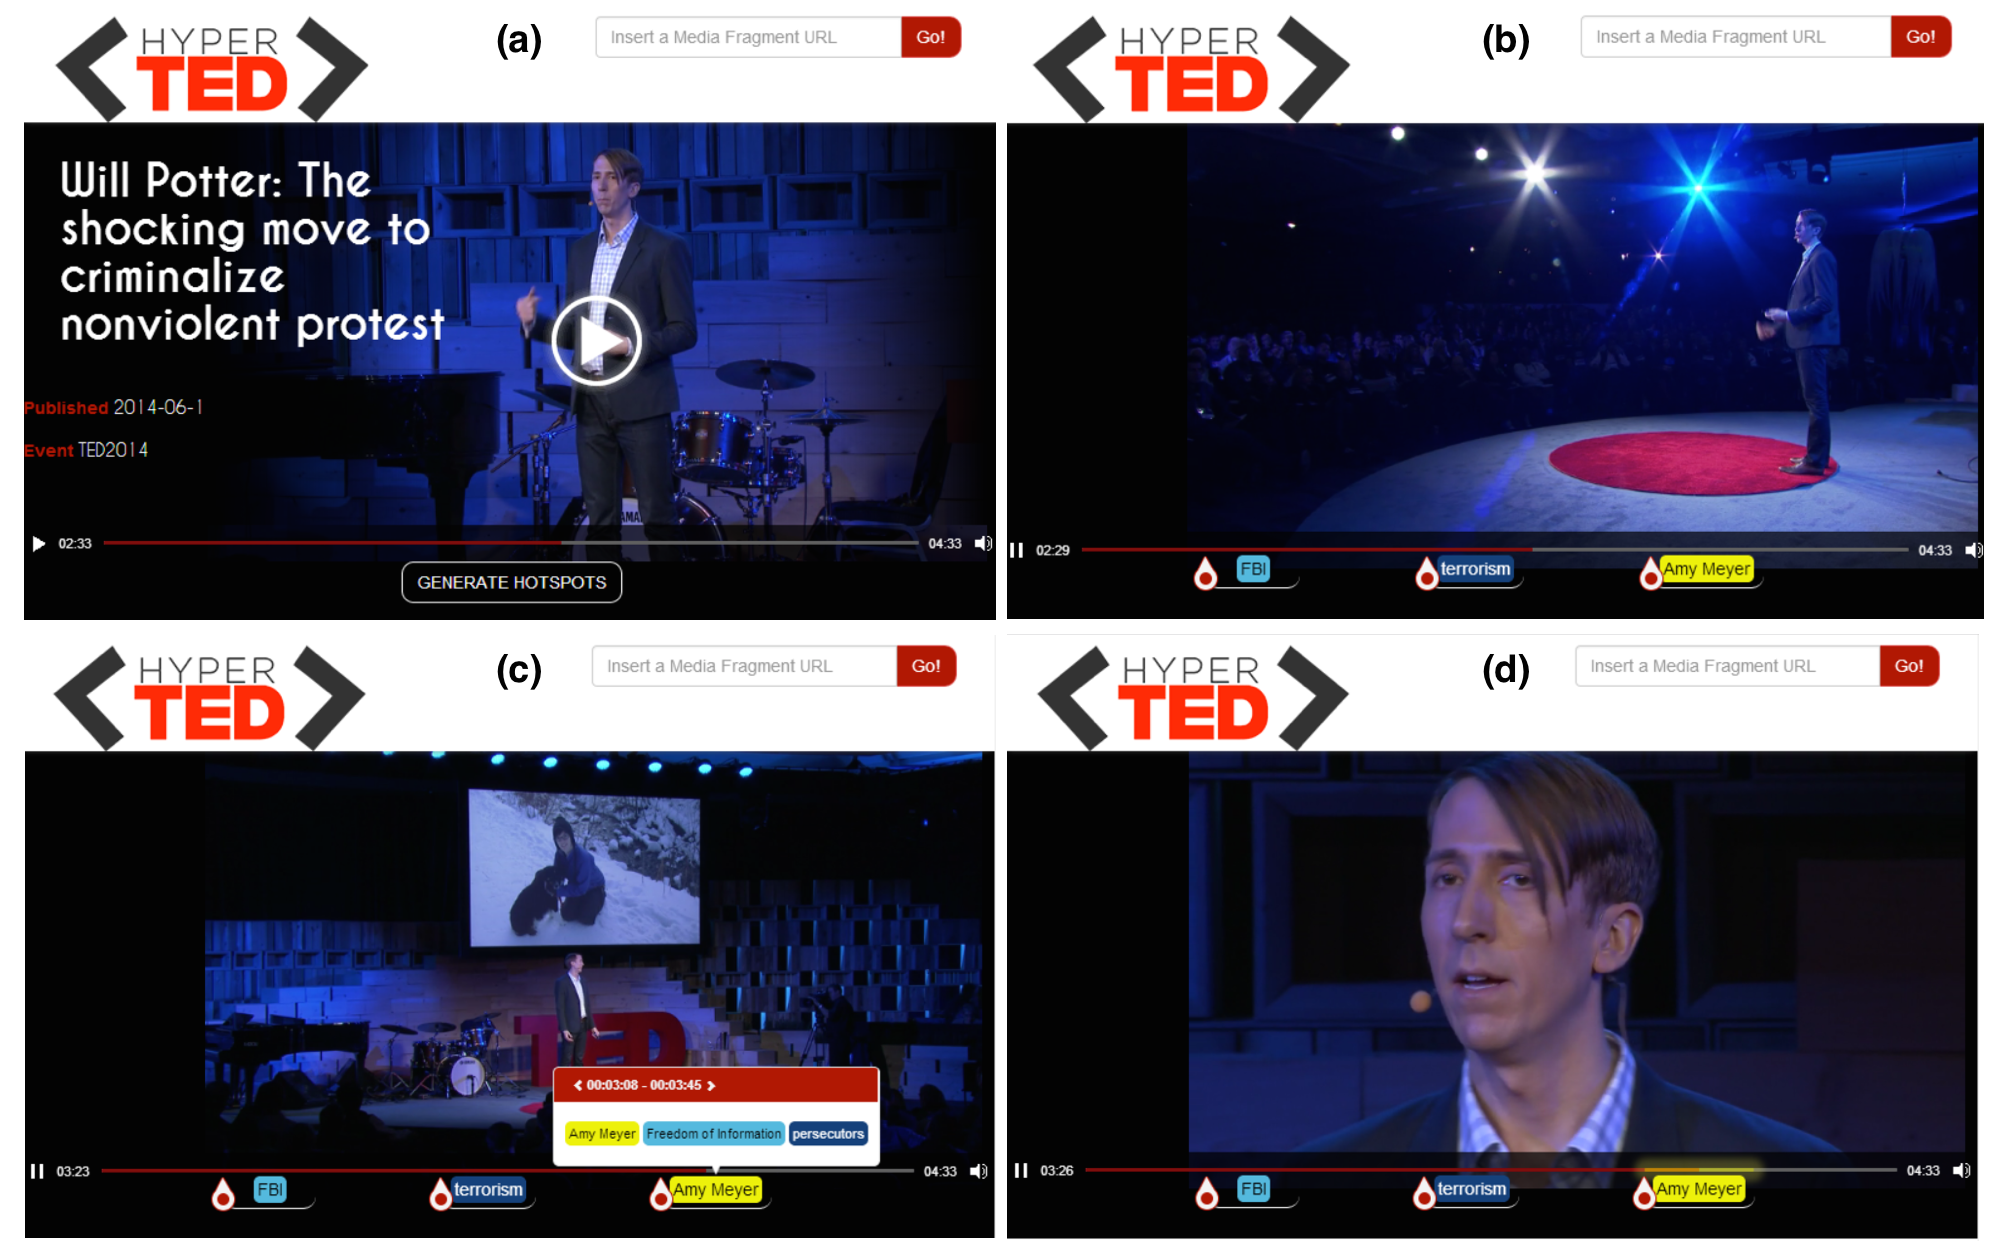
\includegraphics[width=1\textwidth]{figure/Ted_U}
\caption{Visualizing the Hot Spots of a TED Talk (available at \fontsize{8pt}{1em}\selectfont \protect\url{http://linkedtv.eurecom.fr/mediafragmentplayer/video/bbd70fff-e828-4db5-80d0-1a4c9aea430e})}
\label{fig:demoScreenShots}%\end{figure}
\end{figure}


%%%%%%%%%%%%%%%
%% Publications
%%%%%%%%%%%%%%%%

\chapter*{Publications}
\label{sec:publications}
\ifpdf
    \graphicspath{{Chapter2/Chapter2Figs/PNG/}{Chapter2/Chapter2Figs/PDF/}{Chapter2/Chapter2Figs/}}
\else
    \graphicspath{{Chapter2/Chapter2Figs/EPS/}{Chapter2/Chapter2Figs/}}
\fi

The research carried out during this reporting period has lead to the publication of the following scientific papers:

\section*{Conference}
\begin{enumerate}
\setcounter{enumi}{1}

\item Daniel Stein, Alp Oktem, Evlampios Apostolidis, Vasileios Mezaris, Jos\'e Luis, Redondo Garc\'ia, Rapha\"el Troncy, Mathilde Sahuguet, Benoit Huet.:
\textbf{From raw data to semantically enriched hyperlinking: Recent advances in the LinkedTV analysis workflow.}
NEM Summit 2013, Nantes, 28-30 October 2013,www.nem-summit.eu

\item Jos\'e Luis, Redondo Garc\'ia, Rapha\"el Troncy.:
\textbf{Television meets the Web: a Multimedia Hypervideo Experience}.
ISWC2013, 12th International Semantic Web Conference, 21-25 October 2013, Sydney, Australia.

\item Redondo Garc\'ia, Jos\'e Luis; De Vocht, Laurens; Troncy, Rapha\"el; Mannens, Erik; Van de Walle, Rik:
\textbf{Describing and contextualizing events in TV news show}.
WWW 2014, 2nd International Workshop on Social News on the Web (SNOW 2014), April 7, 2014, Seoul, South Korea.

\item Sahuguet, Mathilde; Huet, Benoit; Cervenkova, Barbora; Apostolidis, Evlampios; Mezaris, Vasileios; Stein, Daniel; Eickeler, Stefan; Redondo Garc\'ia, Jos\'e Luis; Troncy, Rapha\"el; Pikora, Lukas:
\textbf{LinkedTV at MediaEval 2013 search and hyperlinking task}.
MEDIAEVAL 2013, Multimedia Benchmark Workshop, October 18-19, 2013, Barcelona, Spain.

\end{enumerate}


\section*{Poster and Demos}
\begin{enumerate}
\setcounter{enumi}{1}

\item Redondo Garc\'ia, Jos\'e Luis; Hildebrand, Michiel; Perez Romero, Lilia; Troncy, Rapha\"el:
\textbf{Augmenting TV Newscasts via Entity Expansion}.
ESWC 2014, Extended Semantic Web conference Demo \& Poster session, May 24-29, 2014, Crete, Greece.

\item Perez Romero, Lilia; Hildebrand, Michiel; Redondo Garc\'ia, Jos\'e Luis; Hardman, Lynda:
\textbf{LinkedTV News: A dual mode second screen companion for web-enriched news broadcasts}.
TVX 2014, ACM International Conference on Interactive Experiences for Television and Online Video, June 25-27, 2014, Newcastle, UK.

\item Jos\'e Luis Redondo Garc\'ia, Mariella Sabatino, Pasquale Lisena, Rapha\"el Troncy:
\textbf{Detecting and Displaying Hot Spots in Web Videos}.
ISWC 2014, International Semantic Web conference Demo \& Poster session, October 19-23, 2014, Riva del Garda, Trentino, Italy.


\end{enumerate}


%%%%%%%%%%%%%%%
%% Participation in Projects and Missions
%%%%%%%%%%%%%%%%

\chapter*{Participation in Projects and Missions}

\section*{LinkedTV}

During this reporting period, we have participated in the EU FP7 LinkedTV project which aims to provides a novel practical approach to Future Networked Media. It is based on four phases: annotation, interlinking, search, and usage of television content. The result intends to make Networked Media more useful and valuable and opens completely new areas of application for Multimedia information on the Web.  

\begin{figure*} [h]
\centering

\includegraphics [scale=0.50] {figure/linkedtv_logo.png}
\caption{LinkedTV Project Logo.}
\label{fig:linkedtv_logo}
\end{figure*} 

\subsection*{Meetings}

We have attended various meetings where we have acquired new ideas and complement our knowledge about this PhD research topics:

\begin{itemize}
\item  LinkedTV plenary meeting in Postdam (28-30 Jan 2014, Postdam, Germany).
\end{itemize}

\subsection*{Deliverables}

We have participated and will be collaborating in the following documents for the Linked TV project:

\begin{itemize}
\item   Deriverable 2.6: \textbf{Advanced concept labelling by complementary Web mining}
\item   Deriverable 2.7: \textbf{Final Linked Media Layer and evaluation}
\end{itemize}


\section*{MediaMixer}

MediaMixer aims to set up and sustain a community of video producers, hosters, and redistributors who will be supported in the adoption of semantic multimedia technology in their systems and workflows to build a European market for media fragment re-purposing and reselling.


\begin{figure*} [h]
\centering

\includegraphics [scale=0.50] {figure/mediamixer_logo.jpg}
\caption{MediaMixer Project Logo.}
\label{fig:linkedtv_logo}
\end{figure*} 


MediaMixer project addresses this deficit by showing the vision of a media fragment market to the European media production, library, TV archive, news production, e-learning and UGC portal industries. We work on 
demonstrating the achievable benefits enabled by the creation, repurposing and reuse of digital contents across borders on the Web, where media fragments are intelligent digital objects, identified and classified at a highly granular degree, integrated with knowledge management, and connected at Web-scale.


\section*{Other Events and Missions}

Apart of the cooperation with the LinkedTV and MediaMixer projects described in the previous sections, we have also participated in the following events:

\begin{itemize}

\item   \textbf{ ESWC 2014 } (24 - 29 May, 2014. Crete, Greece)
\item   \textbf {Research visit to CWI} (2 - 16 Dec, 2013. Amsterdam, the Netherlands)

\end{itemize}


%%%%%%%%%%%%%%%
%% Future
%%%%%%%%%%%%%%%%


\chapter*{Future Guidelines}
\label{future}

After some preliminary results, we have discovered that using techniques like Named Entity Expansion, we can successfully expand the initial set of recognized entities with more relevant concepts not detected by pure named entity recognition approaches. In the same line, Exploring DBpedia paths along the named entities occurring in news media leads to a more accurate ranking of important concepts and even if it does not necessary introduce any new top item, it brings forward more related entities with additional information about the broader context of an event. However, a more formal evaluation is needed in order to test if the developed techniques perform well in a wider variety of situations. In the upcoming weeks we plan to further evaluate the proposed algorithms and tools and compare them with other approaches from the state of the art. 

The cooperation with the AVRO (via Sound and Vision) and RBB broadcasters as partners of the LinkedTV project opens many possibilities to successfully carry out this task. Apart of having more material to be processed, their viewers and editors can potentially test new features and provide feedback about the quality of the annotations and the usefulness of the enrichment process. The evaluation of the entire approach will be based on three complementary dimensions. First, the accuracy of the named entity extraction process, which will be evaluated by applying standard metrics from the NLP domain. Second, we will measure the precision and recall of the search and hyperlinking operations over the generated Media Fragments: for a particular search term given by a user, are the media fragments retrieved relevant? And finally we will study if the links between media fragments are interesting from a user point of view. The evaluation of this part is probably the most subjective and complex one so we will rely on standard datasets like the MediaEval Search and Hyperlinking Task\footnote{\url{http://www.multimediaeval.org/mediaeval2014/}} one, which that has exactly this goal.

Other future work includes a better analysis of the DBpedia properties for detecting the most likely used predicates between context entities. By prioritizing paths using those properties and following them, we should be able to find other relevant entities more easily or to justify the ones that have been previously selected. The adjacency matrix we generate in this phase will be also used for more in depth analysis like topic extraction based on entity clustering. 

%\cleardoublepage
%\addcontentsline{toc}{chapter}{Bibliography}
%\bibliography{biblio}

\end{document}
